\section{Лекция 8}
Введем величину, которая не зависит от времени --- \textbf{вероятность перехода в единицу времени}. Она по определению равна
\[
w_{fi} = \lim\limits_{t \longrightarrow \infty} \dfrac{d W_{fi}(t)}{dt}
\]
Такое определение зачастую работает, т.к. обычно длительность эксперимента сильно больше характерных времен процессов в квантовой системе.\\

На прошлой лекции пришли к двум возможным случаям.
\begin{enumerate}
	\item \[
	\left|\Delta\omega^{(-)}\right| = |\omega_{fi} - \omega| << |\omega_{fi}|
	\]
	$\Longrightarrow$ вторым слагаемым пренебрегаем:
	\[
	W_{fi}^{(-)} = \dfrac{4|F_{fi}|^2}{\hbar^2}\dfrac{\sin{^2\left(\dfrac{\Delta\omega^{(-)}t}{2}\right)}}{(\Delta\omega^{(-)})^2}
	\]
	Переходя к вероятности перехода в единицу времени, получим
	\[
	w_{fi} = \lim\limits_{t \longrightarrow \infty} \dfrac{d W_{fi}(t)}{dt} = \lim\limits_{t \longrightarrow \infty} \dfrac{2|F_{fi}|^2}{\hbar^2}\dfrac{\sin{(\omega^{(-)}t)}}{\Delta \omega^{(-)}} = \Bigg| \text{ т.к. } \lim\limits_{t \longrightarrow \infty} \dfrac{\sin{(\omega t)}}{\pi \omega} = \delta(\omega)\Bigg| = \dfrac{2\pi}{\hbar^2}|F_{fi}|^2\delta(\Delta\omega^{(-)}) =
	\]
	\[
	= \Bigg| \text{ т.к. } \delta(ax) = \dfrac{1}{|a|}\delta(x) \Bigg| = \dfrac{2\pi}{\hbar^2}|F_{fi}|^2\delta(E_f^{(0)} - E_i^{(0)} -\hbar\omega)
	\]
	Это же можно изобразить графически следующим образом:
	\begin{figure}[H]
		\centering
		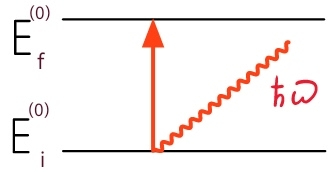
\includegraphics[width=0.4\linewidth]{images/lecture_8_1.jpg}
	\end{figure}
	\item 
	\[
	\left|\Delta\omega^{(+)}\right| = |\omega_{fi} + \omega| << |\omega_{fi}|
	\]
	$\Longrightarrow$ первым слагаемым пренебрегаем:
	\[
	W_{fi}^{(+)} = \dfrac{4|F_{if}|^2}{\hbar^2}\dfrac{\sin{^2\left(\dfrac{\Delta\omega^{(+)}t}{2}\right)}}{(\Delta\omega^{(+)})^2}
	\]
	Переходя к вероятности перехода в единицу времени, получим
	\[
	w_{fi} = \dfrac{2\pi}{\hbar^2}|F_{if}|^2\delta(E_f^{(0)} - E_i^{(0)} + \hbar\omega)
	\]
	Это же можно изобразить графически следующим образом:
	\begin{figure}[H]
		\centering
		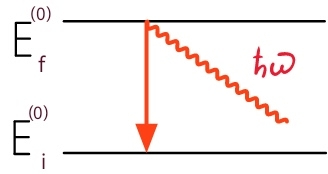
\includegraphics[width=0.4\linewidth]{images/lecture_8_2.jpg}
	\end{figure}
\end{enumerate}

Заметим, что $\hat{F} e^{-i\omega t}$ --- аналог оператора рождения (энергия системы увеличивается на $\hbar \omega$), a $\hat{F}^\dagger e^{-\omega t}$ --- аналог оператора уничтожения (энергия системы уменьшается на $\hbar \omega$).\\

Пусть теперь $\hat{H}_0$ имеет смешанный спектр. Выберем начальное состояние с дискретным уровнем энергии $E_i^{(0)}$. Перейдем в состояние с энергией из непрерывного спектра $E_f$ (непрерывный спектр $\hat{H}_0$ совпадает с непрерывным спектром $\hat{H}$), в таком случае $\hbar\omega > I$ --- энергия ионизации.\\
\begin{figure}[H]
	\centering
	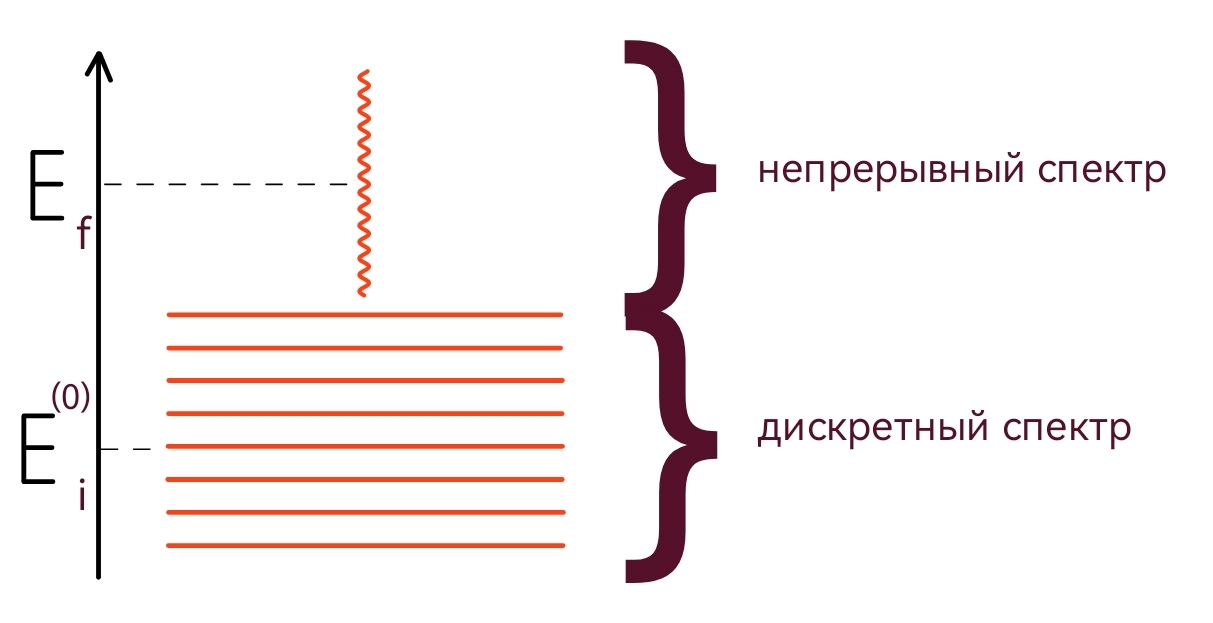
\includegraphics[width=0.75\linewidth]{images/lecture_8_3.jpg}
\end{figure}

В силу нормировки, вероятность перехода в конкретное состояние непрерывного спектра равна нулю. Тогда рассмотрим некоторый отрезок $[E_f,~ E_f + dE_f]$. Тогда ширина узкого уровня $d\Gamma_{E_f} = \rho(E_f)dE_f$. Подставляя это в вероятность прехода в единицу времени, получим
\[
d w_{fi}^{(-)} = \dfrac{2\pi}{\hbar}|F_{fi}(E_f)|^2\delta(E_f - E_i^{(0)} - \hbar\omega)~d\Gamma_{E_f} = \dfrac{2\pi}{\hbar}|F_{fi}(E_f)|^2\delta(E_f - E_i^{(0)} - \hbar\omega)\rho(E_f)~dE_f
\]
Проинтегрируем:
\[
w_{fi}^{(-)} = \dfrac{2\pi}{\hbar}|F_{fi}(E)|^2\rho(E)\Bigg|_{E = E_i^{(0)}+\hbar\omega}
\]
Для свободной частицы в ящике объема $V$
\[
d\Gamma_E = \dfrac{V~d\vec{p}}{(2\pi\hbar)^3} = \rho(E)~dE, \tab \rho(E) = \dfrac{\sqrt{2mE}mV}{(2\pi\hbar)^3}d\Omega
\]

Заметим также, что условие применимости принимает вид
\[
W_{fi} = w_{fi}t << 1
\]












\subsection{\S XIV.1.5 Переходы под действием постоянного возмущения. "Золотое правило"  Э. Ферми. Квазистационарные состояния.}
Сведем переходы под действием периодического возмущения к переходам под действием постоянного. Возмущения постоянно, поэтому $\omega = 0$. Тогда как возникают переходы? Рассмотрим на примерах.

\begin{example}
	Рассмотрим непрерывный спектр гамильтониана: $E > 0$. Пусть система вырождена по квантовому числу $\xi$, и есть невозмущенный гамильтониан $\hat{H}_0$ такой, что $\hat{H}_0\ket{E,~\xi} = E\ket{E,~\xi}$. Начальное состояние, которое задаетс экспериментатором --- $\ket{i} = \ket{E_i,~\xi_i}$, конечное --- $\ket{f} = \ket{E_f,~\xi_f}$.
\end{example}







\subsection{\S XIV.2 Точная теория квантовых переходов.}
\[
\hat{S}(t,~t_0) = \hat{T} \left(e^{-\dfrac{i}{\hbar}\int\limits_{t_0}^t d\tau~\hat{V}^{(I)}(\tau)}\right) = \hat{1} + \hat{\tau}(t,~t_0),
\]
где $\hat{\tau}$ --- оператор перехода. Значит, можно построить теорию по любому порядку $\Longrightarrow$
\[
W_{fi} = \left| \braupket{\psi_f^{(0)}}{\hat{S} = \hat{1} + \hat{\tau}}{\psi_i^{(0)}} \right|^2 = \left| \braupket{\psi_f^{(0)}}{\hat{\tau}(t,~t_0)}{\psi_i^{(0)}} \right|^2 ,
\]
\[
\hat{\tau}(t,~t_0) = \hat{S}(t,~t_0) - \hat{1} = \sum\limits_{\zeta = 1}^\infty \dfrac{1}{\zeta !}\left(-\dfrac{i}{\hbar}\right)^\zeta \int\limits_{t_0}^t d\tau_1~ ... \int\limits_{t_0}^t d\tau_\zeta~ T(\hat{V}^{(I)}(\tau_1)...\hat{V}^{(I)}(\tau_\zeta))
\]



